\documentclass[aspectratio=169,11pt]{beamer}
\usepackage[T1]{fontenc}
\usepackage{lmodern}
\usepackage{amsmath,amssymb,booktabs,graphicx,tikz,array}
\usetikzlibrary{arrows.meta}
\usepackage[backend=bibtex,style=authoryear,sorting=nyt,maxcitenames=2,maxbibnames=4,doi=false,url=false,isbn=false,eprint=true]{biblatex}
\addbibresource{../../refs.bib}
\addbibresource{extra.bib}
\renewcommand*{\bibfont}{\fontsize{6}{7}\selectfont}
\setlength{\bibitemsep}{0.5pt}

\usetheme{default}
\usefonttheme{professionalfonts}
\usefonttheme{serif}
\setbeamertemplate{navigation symbols}{}
\setbeamertemplate{bibliography item}{}
\setbeamertemplate{frametitle continuation}{}
\setbeamertemplate{footline}{\hfill{\tiny\color{gray}\insertframenumber}\hspace{1em}\vspace{0.6em}}
\setbeamertemplate{itemize items}{\textendash}
\newtheorem{proposition}[theorem]{Proposition}
\definecolor{ink}{RGB}{20,32,46}
\setbeamercolor{structure}{fg=ink}
\setbeamercolor{frametitle}{fg=ink}
\setbeamercolor{title}{fg=ink}
\setbeamercolor{block title}{fg=ink,bg=}
\setbeamercolor{block body}{bg=}
\setbeamerfont{frametitle}{size=\large,series=\bfseries}
\setbeamerfont{block title}{series=\bfseries,size=\normalsize}
\setbeamersize{text margin left=2.2em,text margin right=2.2em}
\setlength{\parskip}{0.55em}

\newcommand{\R}{\mathbb{R}}
\newcommand{\E}{\mathbb{E}}
\newcommand{\Prob}{\mathbb{P}}
\newcommand{\one}{\mathbf{1}}
\DeclareMathOperator*{\argmax}{arg\,max}
\DeclareMathOperator*{\argmin}{arg\,min}
\newcommand{\src}[1]{\par\vfill{\scriptsize\color{gray}#1\par}}

\title{Portfolio-Implied Contests,\\ with an Application to Tail Risk}
\author{Peter Cotton}
\date{}

\begin{document}

\begin{frame}
\titlepage
\end{frame}

% ---------------------------------------------------------------- problem
\begin{frame}{The question}
An investor holds a long-only portfolio $w^0 \in \operatorname{int}\Delta$: a
capitalization index, an equal-weight book, any weights that sum to one.

The investor has a view about \emph{dependence}, for example that a group of
names will fall together more often than the benchmark assumes. The view says
nothing about expected returns.

What portfolio $w$ reflects that view and nothing else?

\textcite{black1992} answer the corresponding question for views on returns.
Their reverse step is linear, $\mu = \gamma\,\Sigma\, w^0$. For views on
dependence there is no linear analogue.
\end{frame}

\begin{frame}{Joint declines of the Dow constituents}
\centering
\begin{tabular}{lccc@{\qquad}ccc}
  \toprule
  & \multicolumn{3}{c}{all down by ${>}q$} & \multicolumn{3}{c}{all up by ${>}q$} \\
  \cmidrule(lr){2-4}\cmidrule(lr){5-7}
  $q$ & observed & Gaussian & ratio & observed & Gaussian & ratio \\
  \midrule
  $1.0\%$ & $0.32\%$ & $0.080\%$  & $4$          & $0.24\%$ & $0.111\%$  & $2$  \\
  $1.5\%$ & $0.21\%$ & $0.012\%$  & $18$         & $0.13\%$ & $0.018\%$  & $7$  \\
  $2.0\%$ & $0.11\%$ & $0.0014\%$ & $77$         & $0.05\%$ & $0.0022\%$ & $25$ \\
  $3.0\%$ & $0.05\%$ & ${\sim}0$  & ${>}10^{4}$  & $0\%$    & ${\sim}0$  & n/a  \\
  \bottomrule
\end{tabular}

\raggedright
\medskip
Share of days on which all 28 names move by more than $q$, against a Gaussian
fitted to their means and covariance.

Keeping each empirical marginal and making only the copula Gaussian gives
$5\times10^{-6}$ for the $2\%$ joint decline, against $0.11\%$ observed. The
shortfall is in the dependence.
\src{28 constituents with full 2010--2024 history, about 3{,}770 days, daily log
returns; Gaussian probabilities by $10^8$ draws. The deepest rows rest on two to
four days.}
\end{frame}

\begin{frame}{Tail dependence is not a moment}
The lower-tail dependence coefficient of a pair is
\[
  \lambda_L \;=\; \lim_{u\downarrow 0}\Prob\big(U_i<u \,\big|\, U_j<u\big),
  \qquad U_i = F_i(R_i).
\]
It is zero for every Gaussian copula with correlation below one
\parencite{sibuya1960}.

Two universes with the same covariance have the same minimum-variance,
risk-parity, hierarchical-risk-parity and Schur weights, and may have
different probabilities of a joint crash. Shrinking or re-estimating $\Sigma$
does not separate them.

The evidence that equity dependence is stronger in falling markets is old:
\textcite{longinsolnik2001}, \textcite{angchen2002}, \textcite{poon2004},
\textcite{patton2004}; and \textcite{embrechts2002} on correlation as an
incomplete summary.
\end{frame}

% ---------------------------------------------------------------- prior art
\begin{frame}{Prior art: tilting a benchmark by a view}
\footnotesize
\begin{tabular}{@{}>{\raggedright\arraybackslash}p{0.31\textwidth}>{\raggedright\arraybackslash}p{0.25\textwidth}>{\raggedright\arraybackslash}p{0.40\textwidth}@{}}
  \toprule
  & View is on & From view to weights \\
  \midrule
  \textcite{black1992} & expected returns & linear reverse step, Bayesian update,
     then mean--variance with $\Sigma^{-1}$ \\ \specialrule{0.25pt}{2.5pt}{2.5pt}
  Entropy pooling \parencite{meucci2008} & scenario probabilities; tails
     allowed & minimum relative entropy re-weighting of scenarios, then a
     second optimization \\ \specialrule{0.25pt}{2.5pt}{2.5pt}
  Scenario CVaR \parencite{rockafellar2000} & none (a risk measure) & linear
     program over scenarios \\ \specialrule{0.25pt}{2.5pt}{2.5pt}
  HRP, Schur, HERC \parencite{lopezdeprado2016,cotton2024schur,raffinot2018} &
     none & recursion on a tree cut from the covariance \\ \specialrule{0.25pt}{2.5pt}{2.5pt}
  This paper & the joint law of performances & deterministic inverse at the
     benchmark, then one forward simulation \\
  \bottomrule
\end{tabular}

\normalsize
{\small This paper's method re-solves no program and inverts no covariance. It
can take a Black--Litterman posterior portfolio as its benchmark, which uses both kinds of view.}
\end{frame}

\begin{frame}{Prior art: random-utility choice}
\textcite{thurstone1927}: each alternative has a latent ability and a noisy
performance, and the extreme performance is chosen. \textcite{mosteller1951}
gave the equal-correlation case.

\textcite{luce1959}: the ratio $w_i/w_j$ does not depend on the other
alternatives. Capitalization weighting satisfies this axiom on every
sub-universe. \textcite{yellott1977}: Luce's model is a Thurstone race with
Gumbel performances.

\textcite{williams1977} and \textcite{mcfadden1981}: choice probabilities are
the gradient of the expected maximum utility. The same identity is the
perturbed-optimizer construction of \textcite{berthet2020}.

The Gaussian member of the family, the multinomial probit, lost applied work to
the logit on tractability. Each choice probability is an $(n-1)$-dimensional
orthant integral, simulated one alternative at a time by the GHK method
\parencite{geweke1989,keane1994,hajivassiliou1996}. Recovering abilities from
shares was considered impractical for large $n$.
\end{frame}

% ---------------------------------------------------------------- method
\begin{frame}{The race}
Asset $i$ has an ability $a_i$ and a performance
\[
  X_i = a_i + \varepsilon_i, \qquad \varepsilon \sim S ,
\]
where $S$ is a centred joint law. The lowest performance wins. The weight of an
asset is its winning probability,
\[
  w_i \;=\; W_S(a)_i \;=\; \Prob\big(X_i = \min\nolimits_k X_k\big),
\]
with ties split evenly. Every realization hands out one unit of weight, so
$w\in\Delta$ for any $S$ and any $a$.

Only relative performance matters: $W_S(a + c\,\one) = W_S(a)$.

\begin{lemma}[Calibration]
For a Gaussian reference $S_0 = \mathcal N(0,C_0)$ with $C_0\succ0$, the map
$W_{C_0}:\R^n/\operatorname{span}\{\one\}\to\operatorname{int}\Delta$ is a smooth
bijection. Every strictly positive benchmark has a unique ability vector, up to
an additive constant.
\end{lemma}
\end{frame}

\begin{frame}{The dependence tilt}
\begin{columns}[T,onlytextwidth]
\begin{column}{0.50\textwidth}\setlength{\parskip}{0.5em}
Take a reference law $S_0$ and a target law $S_1$.
\[
  T_{S_0\to S_1}(w^0) \;=\; W_{S_1}\!\big(W_{S_0}^{-1}(w^0)\big).
\]
Abilities are calibrated under the reference and held. The race is run again
under the target.

If $S_1 = S_0$ the benchmark is returned: $T_{S_0\to S_0}=\mathrm{id}$.

Only the reference is inverted. The target enters by forward sampling, so it
may be any simulation: a singular correlation, a Student-$t$, a copula with
lower-tail dependence.
\end{column}
\begin{column}{0.46\textwidth}
\centering
\begin{tikzpicture}[>={Stealth[length=5pt]},x=1cm,y=1cm,font=\small]
  \node (w0) at (0,2.6) {$w^0$};
  \node (w1) at (4.2,2.6) {$w$};
  \node (a0) at (0,0) {$a$ under $S_0$};
  \node (a1) at (4.2,0) {$a$ under $S_1$};
  \draw[->] (w0) -- node[left] {$W_{S_0}^{-1}$} (a0);
  \draw[->] (a0) -- node[below] {hold $a$} (a1);
  \draw[->] (a1) -- node[right] {$W_{S_1}$} (w1);
  \draw[->,dashed] (w0) -- node[above] {$T_{S_0\to S_1}$} (w1);
\end{tikzpicture}

\medskip
\raggedright
Gaussian case, with $\widehat C$ the estimated correlation and
$\phi\in[0,1]$:
\[
  C_1 = (1-\phi)\,C_0 + \phi\,\widehat C .
\]
\end{column}
\end{columns}
\end{frame}

% ---------------------------------------------------------------- engine
\begin{frame}{The inverse: one field for all $n$ assets}
Material from \textcite{cotton2021,cotton2026inversion}. Condition on the winning
value. For independent performances with densities $f_i$ and survival functions
$S_i$,
\[
  p_i \;=\; \int f_i(x)\prod_{j\ne i} S_j(x)\,dx
      \;=\; \int \frac{f_i(x)}{S_i(x)}\;
            \exp\!\Big(\sum\nolimits_{j}\log S_j(x)\Big)\,dx .
\]
The field $\sum_j \log S_j$ is accumulated once on a lattice of $L$ points and
each asset is removed from it in the log domain. All $n$ probabilities cost
$O(nL)$.

GHK returns one probability per run at $O(n^2)$ per draw, with simulation noise
in the value and in its gradient. The integral above is the classical
competing-risks formula; \textcite{domencich1975} wrote it down and judged the
probit case intractable.
\end{frame}

\begin{frame}{Correlation by conditioning}
For a factor covariance $\Sigma = VV^\top + \operatorname{diag}(D)$ the
performances are independent given the factors $f\sim N(0,I_k)$, so
\[
  p(a) \;=\; \sum_{q=1}^{Q} \omega_q\; p^{\mathrm{ind}}\big(a + V f_q\big),
\]
at cost $O(nLQ)$. The quadrature is that of \textcite{butler1982}; the shared
field returns all $n$ probabilities from each node.

\small
\begin{tabular}{@{}ll@{}}
  \toprule
  Model & Covariance \\
  \midrule
  Luce / softmax & independent, Gumbel base \\
  Thurstone--Mosteller & independent, normal base \\
  factor multinomial probit & $VV^\top+\operatorname{diag}(D)$ \\
  sectors, market plus sectors & blocks; blocks with a global factor \\
  hierarchies & tree of shared effects \\
  \bottomrule
\end{tabular}

\normalsize
The hierarchical case contains the covariance structure assumed by hierarchical
risk parity. A dense $\Sigma$ is handled only approximately.
\end{frame}

\begin{frame}{The Jacobian is a graph Laplacian}
Asset $i$ wins on the cone $R_i=\{x: x_i\le x_k\ \forall k\}$. Abilities
translate the density, so the divergence theorem moves
$\partial p_i/\partial a_j$ to the face $F_{ij}$ on which $i$ and $j$ tie ahead
of the field:
\[
  \frac{\partial p_i}{\partial a_j}
  \;=\; \int \varphi_{ij}(t,t)\,
        \Prob\big(X_k>t\ \ \forall k\ne i,j \,\big|\, X_i=X_j=t\big)\,dt
  \;=:\; w_{ij} \;\ge 0 .
\]
Hence $w_{ij}=w_{ji}$, rows sum to zero, and
$(Jh)_i=\sum_{j\ne i} w_{ij}\,(h_j-h_i)$.

\begin{theorem}[Cotton 2026]
Let $\mathcal W(a)=\E\min_i(a_i+\varepsilon_i)$. Then $\nabla \mathcal W = p$ and
$\nabla^2 \mathcal W=-L$, with $L$ the Laplacian of the tie densities.
For $p^\star\in\operatorname{int}\Delta$ the program
$\max_a\,\mathcal W(a)-\langle p^\star,a\rangle$ is strictly concave on
$\one^{\perp}$ and its maximizer is the unique inverse, $p(a^\star)=p^\star$.
\end{theorem}
\end{frame}

\begin{frame}{The iteration, and its cost}
Each sweep is one field pass. It returns $p(a)$ and the own-slopes
$\partial p_i/\partial a_i$, and updates
\[
  a_i \;\leftarrow\; a_i - \alpha\,
  \frac{\log p_i(a) - \log p^\star_i}{\partial \log p_i/\partial a_i},
\]
with a clipped step, then recentres. The Jacobian is never formed. The stopping
rule is $\max_i|\log p_i-\log p^\star_i|<10^{-8}$.

Reported timings on one desktop machine:

\begin{itemize}
\item forward map, rank-one factor: $0.12$, $1.2$ and $18$ seconds at
  $n=10^4,10^5,10^6$;
\item inversion at $n=10^6$: under two minutes independent, about twelve
  minutes with a rank-one factor;
\item GHK is more than a hundred times slower at $n=200$, with measured cost
  growing roughly as $n^{2.9}$.
\end{itemize}

No superiority over GHK is claimed for high-rank dense covariance.
\src{\cite{cotton2026inversion}.}
\end{frame}

% ---------------------------------------------------------------- theory
\begin{frame}{What the race optimizes}
Write $\theta=-a$ and $\eta=-\varepsilon$, and
$G_S(\theta)=\E\big[\max_i(\theta_i+\eta_i)\big]$.

\begin{theorem}[Implied objective]
For $C\succ0$, $G_C$ is convex and $C^\infty$, $w=\nabla G_C(\theta)$, and
\[
  w \;=\; \argmax_{p\in\Delta}\ \big\{\langle\theta,p\rangle-\Omega_C(p)\big\},
  \qquad \Omega_C = G_C^{*} .
\]
\end{theorem}

The first claim is the Williams--Daly--Zachary identity; the second is
Fenchel--Young duality. For a general law $S$ the weights are a selected
subgradient of $G_S$.

Gumbel noise gives $\Omega=\sum_i p_i\log p_i$ and $w=\operatorname{softmax}$,
which ignores dependence. A correlated law gives a penalty that depends on the
correlation, and a tail-dependent law one that depends on the tail.

Locally, $\Omega_{S_0}(w^0+\delta)-\Omega_{S_0}(w^0)-\langle\nabla\Omega_{S_0}(w^0),\delta\rangle
\approx \tfrac12\,\delta^\top[\nabla_\theta w]^{-1}\delta$: a Markowitz-type
quadratic with the inverse choice sensitivity in place of $\Sigma$.
\end{frame}

\begin{frame}{Redundant assets}
\begin{columns}[T,onlytextwidth]
\begin{column}{0.60\textwidth}\setlength{\parskip}{0.5em}
\begin{lemma}[Redundancy]
Replace asset $k$ by two perfect duplicates $k',k''$. Then
$w_{k'}=w_{k''}=\tfrac12 w_k$ and every other weight is unchanged.
\end{lemma}

\begin{proposition}[Monotonicity]
In a Gaussian race, raise any covariance between members of a group $T$, with
variances, abilities and all other covariances fixed. The combined weight of
$T$ weakly decreases and every weight outside $T$ weakly increases.
\end{proposition}

The proposition is an application of \textcite{slepian1962}.

Mean--variance reaches the same split by dividing through a vanishing
eigenvalue. Tree methods reach it discretely, as cluster membership flips.
\end{column}
\begin{column}{0.34\textwidth}
\centering\small
\begin{tabular}{cc}
  \toprule
  $\rho_{12}$ & $w_1+w_2$ \\
  \midrule
  $0$    & $0.667$ \\
  $0.5$  & $0.616$ \\
  $0.9$  & $0.551$ \\
  $0.99$ & $0.516$ \\
  $1$    & $0.500$ \\
  \bottomrule
\end{tabular}

\medskip
\raggedright\scriptsize
Three equal-ability assets. Assets 1 and 2 have mutual correlation $\rho_{12}$;
asset 0 is independent of them.
\end{column}
\end{columns}
\end{frame}

\begin{frame}{Tail consistency}
\begin{columns}[T,onlytextwidth]
\begin{column}{0.47\textwidth}\setlength{\parskip}{0.5em}
\begin{lemma}[Tail consistency]
Let $G$ be a group of equal-ability assets, $M_G=\min_{i\in G}X_i$, and
$Y=\min_{j\notin G}X_j$ independent of $G$. Then $w_G=\Prob(M_G<Y)$, and
\begin{itemize}
\item[(i)] a change in the joint law of $G$ that raises $M_G$ in first-order
  stochastic order does not increase $w_G$;
\item[(ii)] in the comonotone limit $w_G$ is the winning probability of a
  single competitor, whatever $|G|$.
\end{itemize}
\end{lemma}

The object that matters is the law of the group's worst performance, which is
set by the lower-tail copula.
\end{column}
\begin{column}{0.50\textwidth}\setlength{\parskip}{0.5em}
\centering
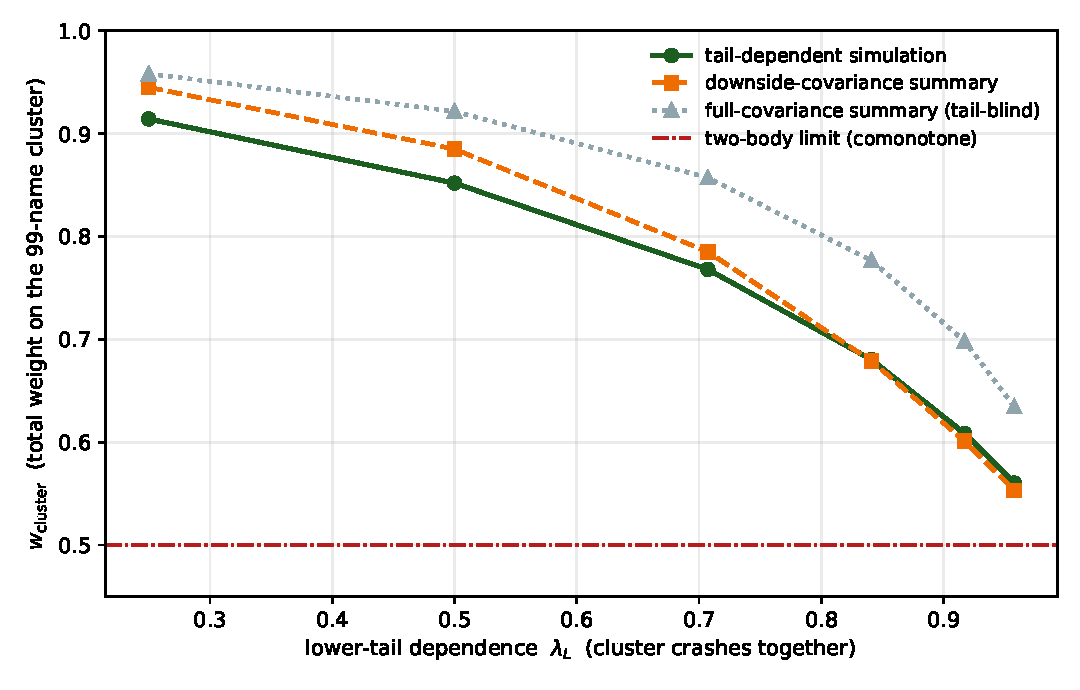
\includegraphics[width=\textwidth]{../figures/tail_consistency.pdf}

\raggedright\scriptsize
One independent asset against a 99-name cluster with Clayton lower-tail
dependence $\lambda_L$ and standard-normal margins. The cluster's combined
weight falls from $99/100$ toward $\tfrac12$. A Gaussian race driven by the
downside semicovariance recovers most of the effect; the full covariance does
not.
\end{column}
\end{columns}
\end{frame}

\begin{frame}{Smoothness in the correlation}
\begin{theorem}[Smoothness]
On positive-definite correlation matrices $w(C)$ is $C^\infty$ in $C$ and in
$a$. If $C_0$ and $C_1$ have smallest eigenvalue at least $\lambda>0$, then
\[
  \|w(C_1)-w(C_0)\|_1 \;\le\; \frac{1}{\sqrt2\,\lambda}\,\|C_1-C_0\|_F
\]
uniformly in the abilities. The order $1/\lambda$ cannot be improved in general.
\end{theorem}

The bound is on the target weights. It limits the turnover caused by a change
in the estimated correlation between rebalances.

The winning regions do not depend on $C$ and partition the sample space. The
derivative of $w$ in a direction $H$ is the expectation of the Gaussian score
over each region, and the score has second moment
$\tfrac12\|C^{-1/2}HC^{-1/2}\|_F^2$.

The finite Monte Carlo estimator is a step function of its inputs. Fixed seeds
keep it stable between rebalances; the theorem is about the population map.
\end{frame}

% ---------------------------------------------------------------- evidence
\begin{frame}{Dow walk-forward, 2010--2024}
\centering
\begin{tabular}{lccc}
  \toprule
  Method & Turnover & Sharpe & Net Sharpe \\
  \midrule
  Equal weight              & $0.004$ & $0.94$ & $0.93$ \\
  Inverse variance          & $0.006$ & $0.95$ & $0.93$ \\
  Risk parity               & $0.005$ & $0.97$ & $0.95$ \\
  Minimum variance          & $0.046$ & $0.88$ & $0.70$ \\
  Hierarchical risk parity  & $0.035$ & $0.97$ & $0.85$ \\
  Schur ($\gamma=0.5$)      & $0.071$ & $0.95$ & $0.70$ \\
  Dependence tilt           & $0.008$ & $0.91$ & $0.89$ \\
  \bottomrule
\end{tabular}

\raggedright
\medskip
The tilt turns over four to nine times less than hierarchical risk parity,
minimum variance and Schur. Of its $0.008$, the motion of the targets is
$0.007$.

Its gross Sharpe is below every method in the table except minimum variance.
Equal weight, inverse variance and risk parity turn over less and have higher
net Sharpe.
\src{28 constituents, daily updates, one-factor market reference, the same
covariance estimate for every method. Turnover is the mean one-way fraction of
the book traded per day. Net Sharpe charges 10 basis points per side.}
\end{frame}

\begin{frame}{Fit time}
\centering
\begin{tabular}{lcccc}
  \toprule
  $n$ & dense min.\ variance & race ($k=5$) & factor min.\ variance & HRP \\
  \midrule
  $250$  & undefined & $0.38$ & $0.01$ & $0.02$ \\
  $1000$ & undefined & $0.90$ & $0.20$ & $0.33$ \\
  $3000$ & undefined & $3.0$  & $1.4$  & $3.2$  \\
  \bottomrule
\end{tabular}

\raggedright
\medskip
Seconds, on five-factor data with a 250-day window. $\Sigma^{-1}\one$ is
undefined once $n\ge T$. The factor-form race and the Woodbury factor optimizer
remain well posed; the factor optimizer is faster.

The path budget is held at $M=2^{16}$, which is why the time is linear in $n$.
The standard error of a weight is about $\sqrt{w_i/M}$ and the weights are of
order $1/n$, so relative precision degrades like $\sqrt{n/M}$. Holding it fixed
means growing $M$ with $n$.
\end{frame}

\begin{frame}{What is not shown}
There is no out-of-sample test that the tail-aware tilt improves drawdown or
expected shortfall. The tail results are the tail-consistency lemma and a simulated example.

On the Dow the tilt has no Sharpe advantage. The measured benefit is turnover
relative to the covariance-inverting and tree methods.

The race sees relative performance. A shock common to every asset leaves the
weights unchanged; a response requires losses that fall on some names relative
to others.

The reference law and the confidence $\phi$ are chosen by the user, and the
paper gives no rule for choosing them.

The weights are winning probabilities, so the method is long-only and fully
invested.
\end{frame}

\begin{frame}{Demonstration and sources}
\begin{columns}[c,onlytextwidth]
\begin{column}{0.56\textwidth}
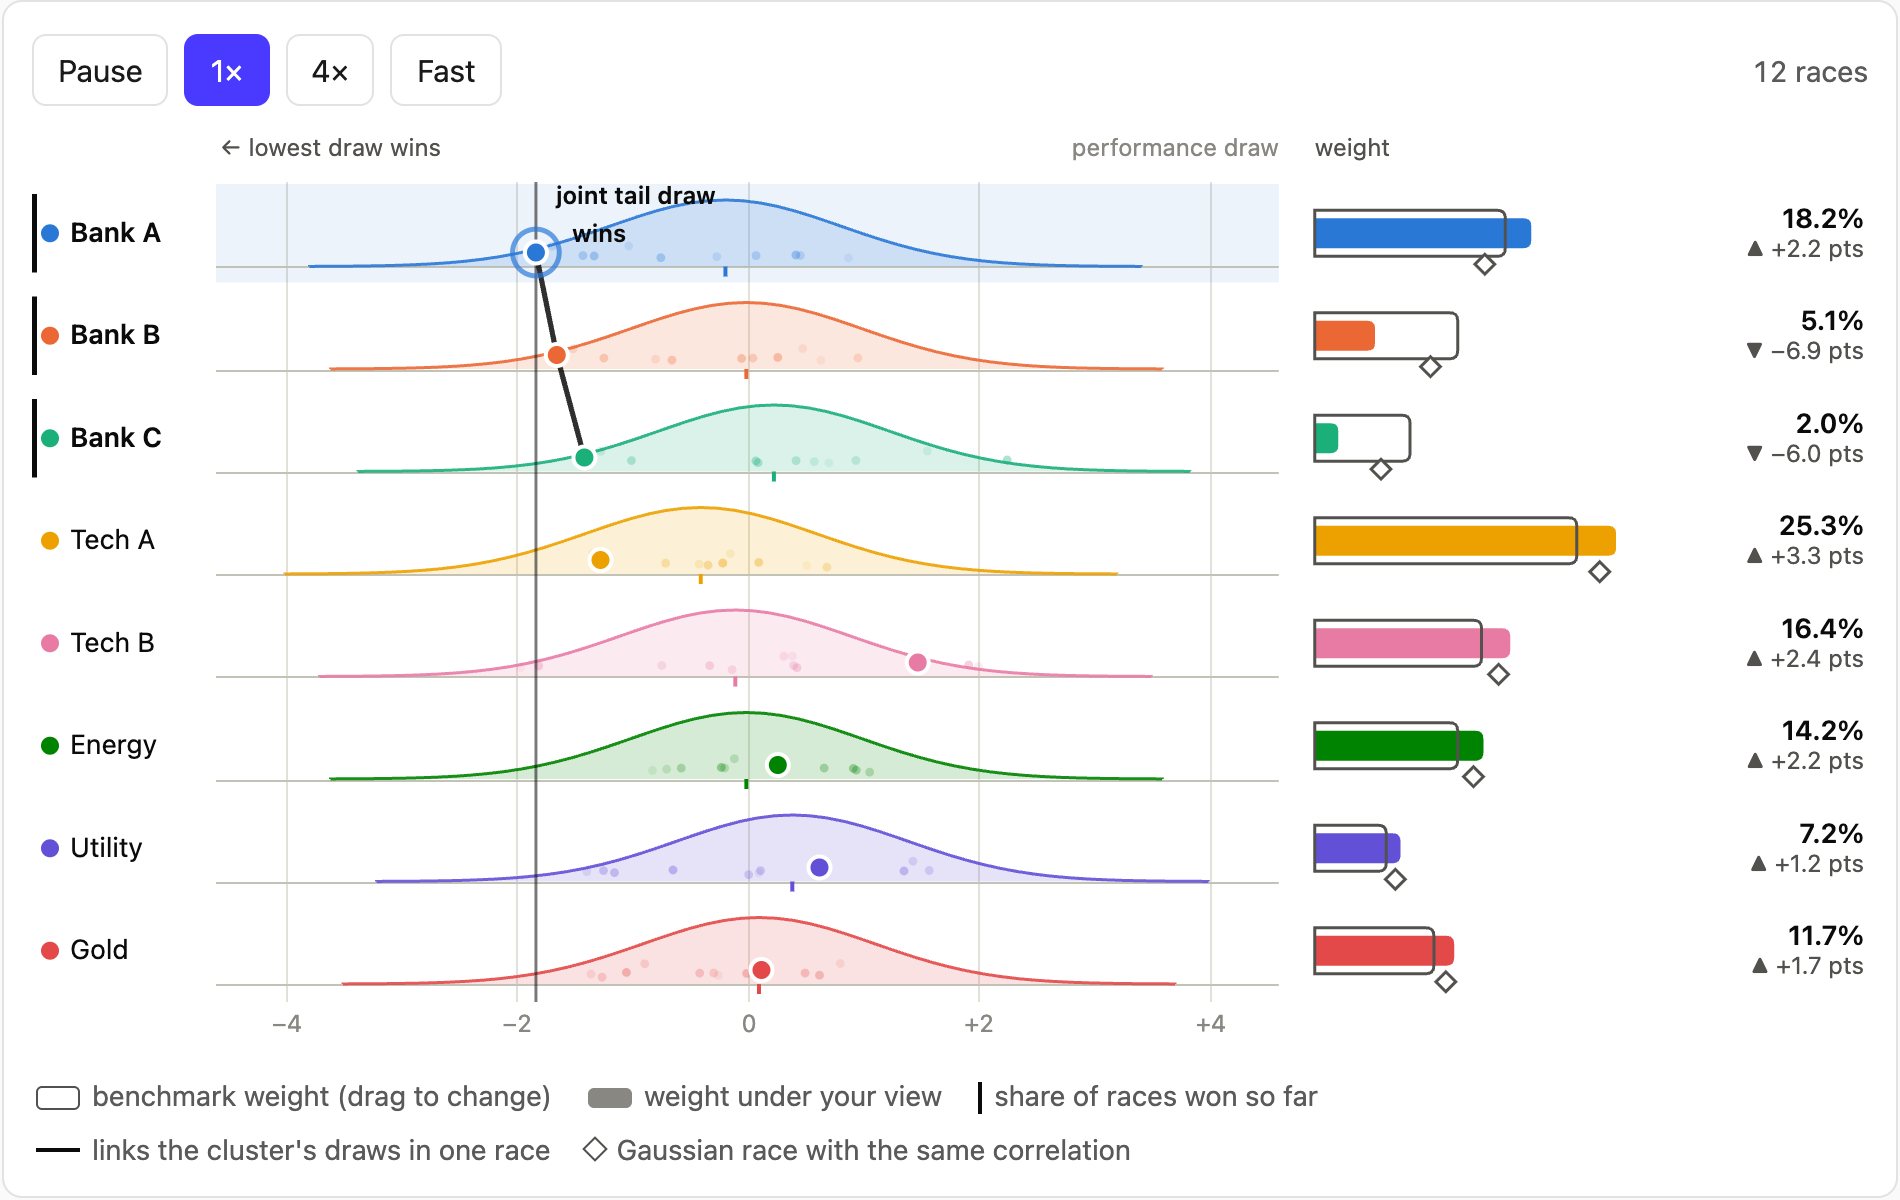
\includegraphics[width=\textwidth]{race_demo.png}
\end{column}
\begin{column}{0.40\textwidth}\setlength{\parskip}{0.5em}
\small
Eight assets in the browser. The three banks share one extreme draw on a share
of races; their combined weight falls from $36.0\%$ to $25.2\%$.

The demonstration uses a simple joint-tail construction and an independent
reference, not the Clayton copula of the paper.

\medskip
\footnotesize
\texttt{allocation.microprediction.org}\\
\texttt{ssrn.com/abstract=7737202}\\
\texttt{github.com/microprediction/allocation}\\
\texttt{github.com/microprediction/winning}
\end{column}
\end{columns}
\end{frame}

\begin{frame}[allowframebreaks]{References}
\printbibliography[heading=none]
\end{frame}

\end{document}
